\subsection{Geração de biomas no diagrama de Voronoi}

Biomas são regiões ecológicas que possuem uma fauna e flora com atributos estruturais semelhantes \cite{maestrovirtuale}. Segundo \citeonline{amitp2010} o primeiro passo para gerar o mapa e os biomas é gerar o litoral, os litorais serão as bordas que irão dizer o que é água e o que é solo. Existem algumas formas de gerar o formato da ilha:

\begin{itemize}
    \item Radial: gera ilhas circulares através de ondas senoidais.
    \item Perlin: utiliza o Perlin Noise para controlar a forma da ilha.
    \item Quadrado: preenche o mapa inteiro com solo.
\end{itemize}

É possível utilizar qualquer formato para gerar as ilhas \cite{amitp2010}, neste trabalho será utilizado o resultado da segmentação de imagem para gerar a ilha.

\begin{figure}[H]
	\caption{Diagrama de Voronoi separado em solo e mar}
	\centering % para centralizarmos a figura
	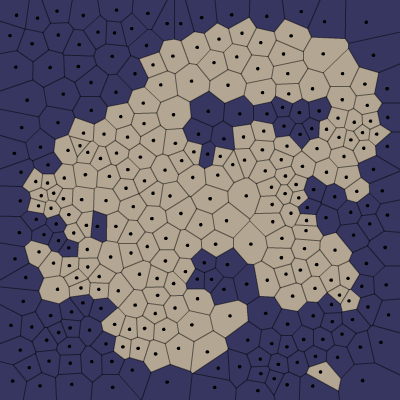
\includegraphics[width=0.8\textwidth]{figures/voronoi-land-water.png} % leia abaixo
	\legend{Fonte: \citeonline{amitp2010}}
	\label{fig:voronoi-land-water}
\end{figure}

O proximo passo é calcular a elevação do terro. A elevação será calculada através da distancia de um polígono indicado como solo até o litoral, a elevação é definida pelos cantos dos polígonos \cite{amitp2010}. 

\begin{figure}[H]
	\caption{Diagrama de Voronoi separado em solo e mar com os cantos dos polígonos indicando a direção para o litoral}
	\centering
	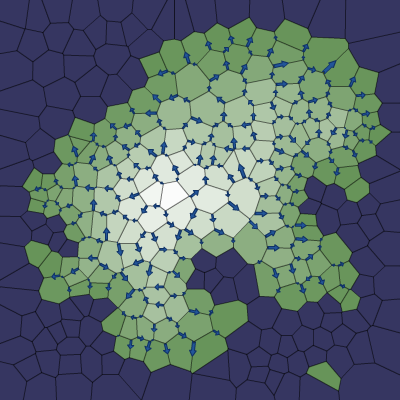
\includegraphics[width=0.7\textwidth]{figures/downslopes.png}
	\legend{Fonte: \citeonline{amitp2010}}
	\label{fig:downslopes}
\end{figure}

Com a elevação é possível gerar os biomas, um exemplo seria elevações altas significa que é uma montanha, logo ela deve possuir neve. Adicionando mais uma camada, além da elevação, como a de umidade, podemos gerar uma variedade maior de biomas. A umidade é calculada de quão longe o polígino está de um corpo d'água.

\subsection*{Diagrama de Whittaker}

O diagrama de Whittaker é uma forma de dividir os terrenos gerados a partir da técnica de geração procedural, esse diagrama inclui valores de temperatura e umidade para separar os biomas \cite{wikidotwhittakerdiagram}.

\begin{figure}[H]
	\caption{Diagrama de Whittaker}
	\centering
	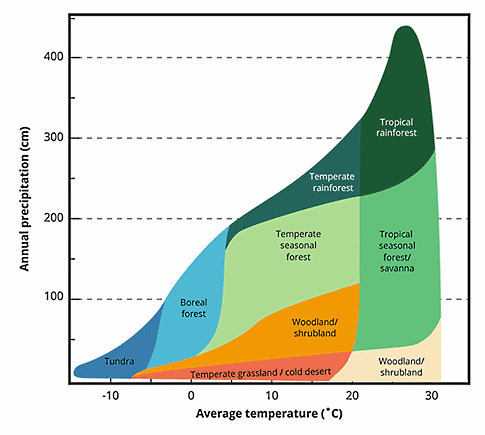
\includegraphics[width=0.6\textwidth]{figures/diagrama-whittaker.png}
	\legend{Fonte: \citeonline{mendes2019}}
	\label{fig:diagrama-whittaker}
\end{figure}

Usando a elevação como representante da temperatura de um bioma é possível utilizar o diagrama de Whittaker, fazendo alterações nesse diagrama é possível adicionar ou remover biomas. Com essa nova camada possibilita a adição de rios ao mapa \cite{amitp2010} e assim obtendo o resultado apresentado na figura \ref{fig:biomes}.

\begin{figure}[H]
	\caption{Resultado final da geração do mapa}
	\centering
	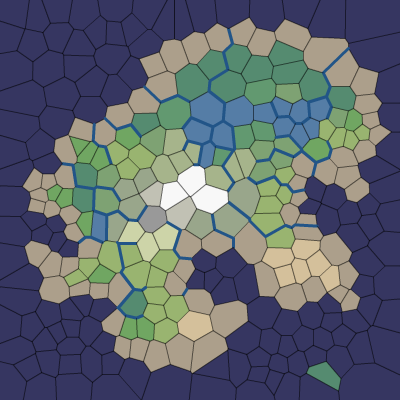
\includegraphics[width=0.5\textwidth]{figures/biomes.png}
	\legend{Fonte: \citeonline{amitp2010}}
	\label{fig:biomes}
\end{figure}


